% !TeX root = ../mde-presentation.tex

\section{Session Introduction} \label{sec:session-intro}

\begin{frame}
	\frametitle[Session title page]{}
	\begin{center}
		{\color{black}
			\textbf{
				\fontsize{36pt}{38pt}\selectfont Modern Earth system science visualization and exploration techniques\\
				\vspace{1.5cm}}}
		\textbf{
			\fontsize{26pt}{28pt}\selectfont The balancing act between complex information, broad functionality and simple illustration \\
		}
		\vspace{1em}
		{\fontsize{18pt}{20pt}\selectfont
            ESSI4.1 | \location \, | \presentationdate \\
			\vspace{1em}
			Conveners: \\
            Tobias Kerzenmacher, Christof Lorenz, Ugur Cayoglu, \textbf{Philipp S. Sommer}}

	\end{center}

    \begin{textblock*}{\textwidth}(0.1\textwidth,0.95\textheight)
        \begin{tabular}{p{0.3\textwidth}p{0.3\textwidth}p{0.3\textwidth}}
            \href{https://kit.edu}{
\includegraphics[width=5cm]{figures/kit.pdf}} &
            \href{https://datahub.erde-und-umwelt.de}{
\includegraphics[width=5cm]{figures/datahub.png}} &
            \hyperlink{frm:map}{
\includegraphics[width=5cm]{figures/hereon.png}}
        \end{tabular}
    \end{textblock*}
\end{frame}

\begin{frame}{Challenges and opportunities}
    \begin{columns}[T]
        \begin{column}{0.45\linewidth}
            Earth system science data are getting increasingly important
            \begin{itemize}
                \item as decision support for stakeholders
                \item for other end users far beyond the scientific domains
                \item within project collaborations
                \item Institutes, Groups and projects are reviewed with respect
                    to the data products they publish
            \end{itemize}
        \end{column}
        \begin{column}{0.45\linewidth}
            But higher temporal and spatial resolutions of modeling and
            remote sensing approaches lead to ever-increasing data
            complexity and volumes

            \vspace{1em}

            \begin{alertblock}<2->{We want to prevent}
                \begin{itemize}
                    \item data that cannot be found
                    \item outdated and insecure software
                    \item always reinventing the wheel
                \end{itemize}
            \end{alertblock}

        \end{column}
    \end{columns}

    \begin{textblock*}{\textwidth}(0.05\linewidth, 1.07\textheight)
		\slidebuttons
	\end{textblock*}

\end{frame}

\begin{frame}{Data standards}
    Making data available can push the use of data standards that improve data
    findability, accessibility, interoperability and reusability (FAIR).

    \vspace{1em}

    \begin{columns}[T]
        \begin{column}<2->{0.6\textwidth}
            \begin{block}{Tool tips to improve data management}
                \begin{itemize}
                    \item use OGC standards for visualization
                    \item do not only visualize, provide download as well
                    \item correctly cite the data and publications you are showing
                    \item ask supplied data to fulfill certain metadata standards
                    \item provide instructions (e.g. in form of Standard Operating Procedures) on how to get different data into your software
                \end{itemize}
            \end{block}
        \end{column}
        \begin{column}{0.3\textwidth}
            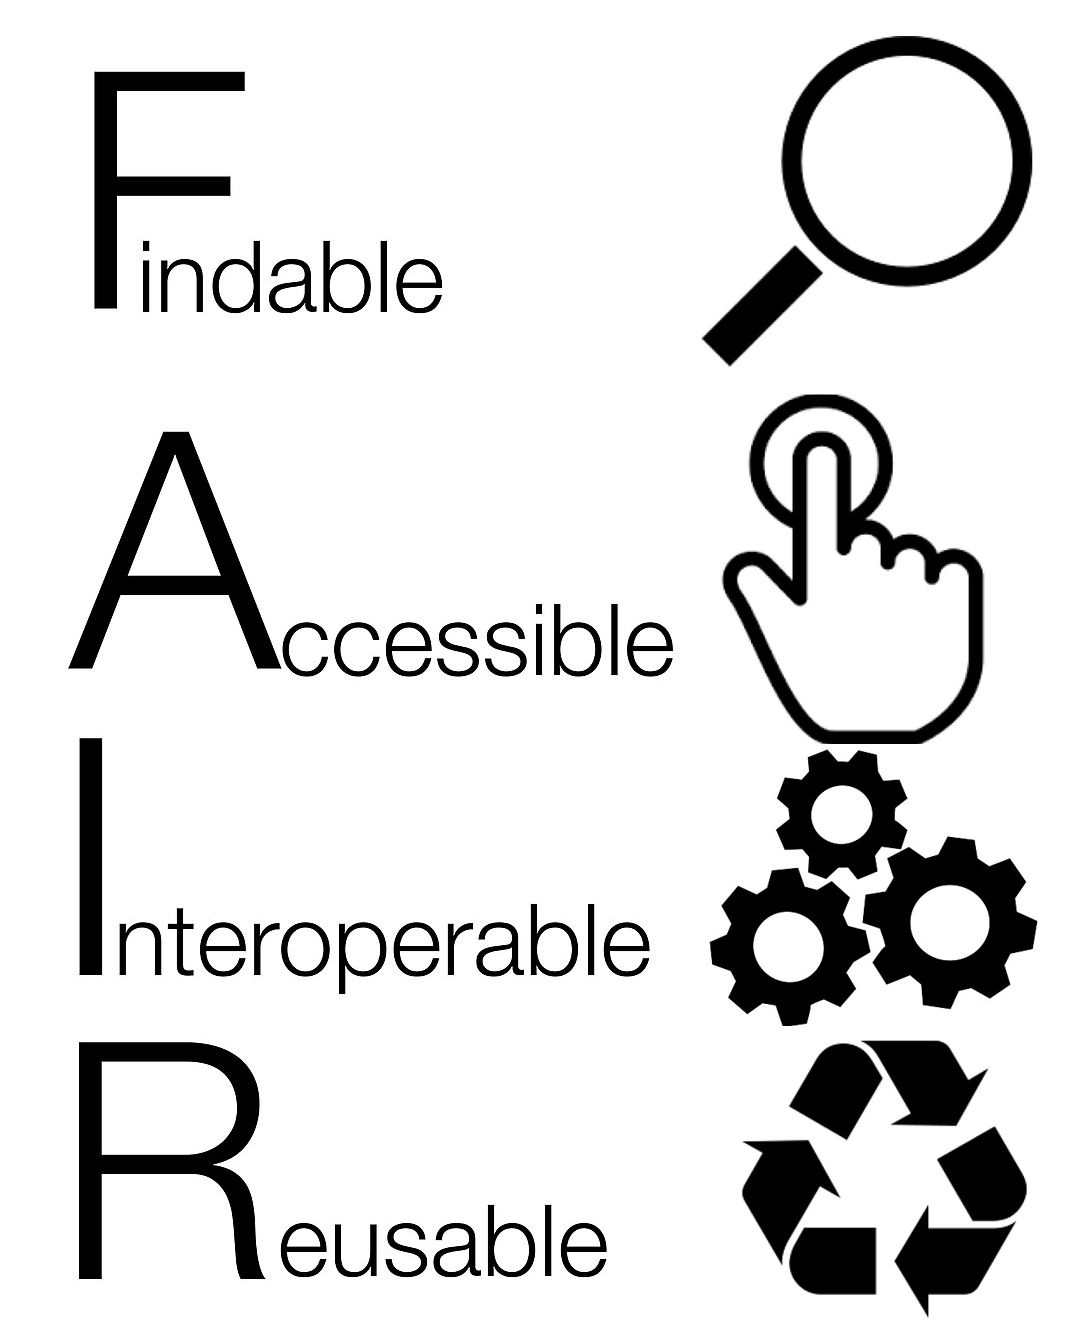
\includegraphics[width=\textwidth]{figures/FAIR_data_principles.jpg}
        \end{column}
    \end{columns}

    \begin{textblock*}{\textwidth}(0.05\linewidth, 1.07\textheight)
		\slidebuttons
	\end{textblock*}

\end{frame}

\begin{frame}{Research Software Recommendations}

    \begin{textblock*}{0.35\linewidth}(0.7\linewidth, 0.23\textheight)
        \slidebuttons
    \end{textblock*}

    \begin{columns}[t]
        \begin{column}{0.5\textwidth}
            \begin{block}{Tips for improving persistence}
                \begin{itemize}
                    \item make your software modular
                    \item invest time in the conceptualization of a software
                        framework
                    \item make it open-source
                    \item make it available in an open gitlab or on github
                    \item make your software installable in different infrastructures
                    \item package your software
                    \item version your software
                    \item containerize your software deployment-ready
                    \item provide login via eduGAIN or other AAI
                \end{itemize}
            \end{block}
        \end{column}
        \begin{column}{0.5\textwidth}
            \begin{block}<2->{Tips for implementing tests}
                \begin{itemize}
                    \item invest time in unit tests
                    \item invest time in stakeholder tests
                    \item automate your documentation
                    \item use continuous integration for testing your software
                \end{itemize}
            \end{block}
            \begin{block}<3->{Tips for documentation}
                \begin{itemize}
                    \item invest time in API documentation
                    \item describe your framework
                    \item provide detailed installation instructions
                \end{itemize}
            \end{block}
        \end{column}
    \end{columns}

\end{frame}

\begin{frame}[t]{Our session}
    A diverse set of tools that make Earth System Science Data available on the
    web

    \vspace{1em}

    \begin{itemize}
        \item Generic data exploration frameworks
        \item Personalized data exploration frameworks driven by a specific
            scientific use-case
        \item Transfer- and outreach-driven exploration frameworks
    \end{itemize}

    \vspace{1em}

    \begin{block}{Our hope}
        Establish a transdisciplinary community of scientists,
        software-developers and other experts in the field of data
        visualization in order to exchange and to give a state-of-the-art
        overview of tools, interfaces and best-practices.
    \end{block}
\end{frame}
